\chapter{Projekt serwisu}
\thispagestyle{chapterBeginStyle}

W tym rozdziale przedstawiono szczegółowy projekt systemu w notacji UML uwzględniający wymagania funkcjonalne opisane we wstępie. Do opisu relacji pomiędzy składowymi systemu wykorzystano diagramy UML.

\section{Struktura}

W serwisie wykorzystano architekturę klient-serwer. Istnieje jeden serwer, do którego może podłączać się wiele klientów i odpowiada on za komunikację i zarządzanie danymi.
W komponencie klienta wykorzystano architekturę trójwarstwową. Architektura ta dzieli komponent na trzy osobne części:
\begin{itemize}
	\item warstwa prezentacji,
	\item warstwa biznesowa,
	\item warstwa danych.
\end{itemize}
Warstwa prezentacji jest to interfejs graficzny użytkownika. Jest odpowiedzialna za interakcję z użytkownikiem (wyświetlanie i wprowadzanie danych). \\ \\
Warstwa biznesowa odpowiada za przetwarzanie komunikatów od użytkownika lub ze strony serwera. Tutaj zawarta jest wszelka logika aplikacji. Przetworzone dane są przekazywane do warstwy prezentacji i/lub warstwy danych. Warstwa ta jest łącznikiem pomiędzy warstwą prezentacji, a warstwą danych. \\ \\
Warstwa danych jest dostępem do danych. Obsługuje połączenie aplikacji z zewnętrznym obiektem dostarczającym dane (baza danych, serwer).

\section{Przypadki użycia}

\begin{figure}[h!]
	\begin{center}
		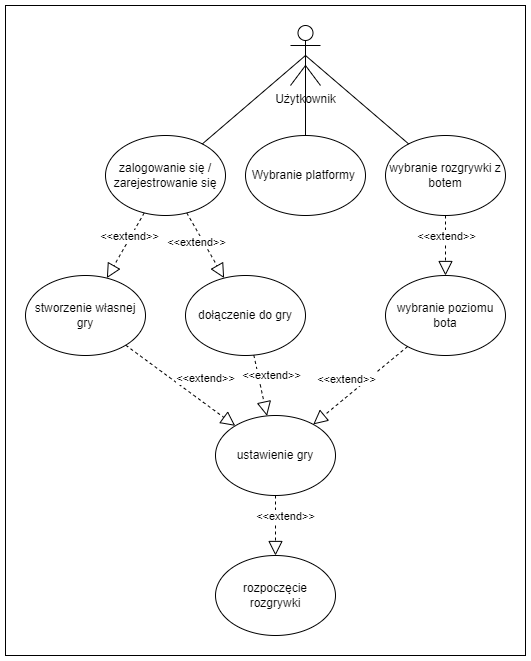
\includegraphics[width=10cm,height=12cm]{img/przypadki-uzycia.png}
	\end{center}
	\caption{{\color{dgray} Diagram przypadków użycia.}} 
	\label{przypadki_uzycia}
\end{figure} 

Użytkownik może wybrać na jakiej platformie będzie chciał korzystać z serwisu. Ma do wyboru stronę internetową albo aplikacje na telefon. Aby móc dołączyć do gry z innymi graczami należy zalogować się lub zarejestrować w aplikacji. Następnie gracz ma możliwość stworzenia własnej gry lub dołączenia do innej. Jeśli zdecyduje się stworzyć własną grę, musi wybrać od 2 do 4 osób spośród wszystkich aktywnych graczy. Dalej przechodzi do panelu konfiguracji gry. Wybiera dozwolony czas na wykonanie ruchu oraz liczbę graczy, jeśli zdecydował się na dołączenie do innej gry. Dołączenie do innej gry działa na zasadzie znalezienia oczekującej gry o takich samych ustawieniach jakie wprowadził gracz. W przypadku nie znalezienia takiej gry jest tworzona nowa gra. Jeśli wszystkie miejsca w grze zostały wypełnione rozgrywka się rozpoczyna. W przypadku wybrania z gry z botem, odbywa się ona lokalnie bez łączenia z serwerem. Użytkownik ma do dyspozycji dwa poziomy bota. Następnie również konfiguruje grę i rozpoczyna rozgrywkę.

\section{Diagramy aktywności}


\section{Diagramy stanów}




